\documentclass[12pt]{article}

\usepackage{cite}
\usepackage{listings}
\usepackage{times}
\usepackage{color}
\usepackage{url}
\usepackage{multirow}
\usepackage{enumitem} % Use for enumerating A, B, C etc...
\urlstyle{same} % Used for formatting formatting url footnotes
\usepackage{fancyhdr} % Header
%\usepackage[table]{xcolor}% http://ctan.org/pkg/xcolor
\usepackage[table,xcdraw]{xcolor}
\usepackage{soul} % highlighting
%\usepackage{pgfgantt} % Project timeline
\usepackage[titletoc,toc,title]{appendix} % Need for appendix, page numbering
\usepackage{tikz}
\usetikzlibrary{calc,arrows.meta,fit,positioning}
%\usepackage{amssymb,graphicx} % Events and milestones
\usepackage{amsmath}
\usepackage{mathtools}
\usepackage{bbm}
\usepackage{amssymb}
\usepackage{booktabs} % used for \toprule in tables
\usepackage{wrapfig,booktabs} % Wrap text around table
\usepackage{booktabs} % used for \toprule in tables
\usepackage[table,xcdraw]{xcolor}
\DeclarePairedDelimiter\ceil{\lceil}{\rceil}
\DeclarePairedDelimiter\floor{\lfloor}{\rfloor}      
\usepackage[final]{pdfpages}
\usepackage{tocloft} % Table of contents spacing
\usepackage{xcolor,colortbl} %%% Color Table Header

\usepackage{makecell}

%\usepackage{subcaption} % Side by side images
%\usepackage{pgfplots} % Bar chart. Graph

\usepackage{xspace} % Needed for et al.
%\newcommand{\etal}{{et al.\@\xspace}} 
\newcommand{\etal}{\emph{et~al.}\xspace} 

\usepackage[bottom=1in, left=1in, right=1in, top=1in]{geometry} 

\usepackage[english]{babel}
\usepackage[utf8x]{inputenc}
\usepackage{graphicx}
\usepackage{wrapfig}
%\usepackage{lipsum}
%\usepackage{pgfgantt}

%\usepackage{minted} % Side by side code


% DK 10/30 Look at removing these
\usepackage[textwidth = 155mm]{geometry}
\usepackage{tabularx}


\newcommand{\todo}[1]{\textcolor{cyan}{\textbf{[#1]}}}
\newcommand{\dan}[1]{\textcolor{blue}{{\it [Dan says: #1]}}}
\newcommand{\qi}[1]{\textcolor{red}{{\it [Qi says: #1]}}}
\newcommand{\sakshi}[1]{\textcolor{green}{{\it [Sakshi says: #1]}}}


%%% Start column formatting
% Note: In overleaf sometimes columns fail to render. Check on PDF Output
\newcolumntype{L}[1]{>{\raggedright\arraybackslash}m{#1}} % raggedright= align left
\definecolor{Gray}{gray}{0.80} % the lower the #, the darker it gets
%%% End Table formatting

%%%% Start toggling showing/hiding some information
\newif\ifShowAll
\ShowAlltrue % Display All Info
%\ShowAllfalse % Hide Some Info

% Uncertainty Reduction Tactic Prediction Mechanism in Self-Adaptive Systems to Reduce System Uncertainty

% Reducing Uncertainty in Self-Adaptive Systems Through the Use of Uncertainty Reduction Tactics
% A XXXX Framework for Reducing Uncertainty in Self-Adaptive Systems

% Integrating Uncertainty Reduction into the Self-Adaptive Control loop

% Increasing the Resiliency and Effectiveness of Self-Adaptive Systems Through the Use of Uncertainty Reduction Tactics

% Developing, Integrating and Evaluating a XXX Decision Support Process for Uncertainty Reduction Tactics in Self-Adaptive Systems

% Using XXXX to Incorporate Uncertainty Reduction Tactics in Self-Adaptive Systems

% Including Uncertainty Reduction Tactics in Self-Adaptive Systems Using XXXXXXX

% Uncertainty Reduction Tactics in Self-Adaptive Systems to Support System Effectiveness, Resiliency and Completion of Mission Critical Objectives

% A XXXX Process for Uncertainty Reduction Tactics in Self-Adaptive Systems

% Enabling Self-Adaptive Systems to be more Resilient, Efficient and Effective Through the Use of Uncertainty Reduction Tactics

% Enabling More Resilient, Efficient and Effective Self-Adaptive Systems Through the Use of Uncertainty Reduction Tactics

% XXX Decision Support for Uncertainty Reduction Tactics
% Prediction Models for Uncertainty Reduction Tactics

% A XXXX Process for Uncertainty Reduction Tactics in Self-Adaptive Systems 

% XXXX for Uncertainty Reduction Tactics in Self-Adaptive Systems

% Bayesian dynamic matrix factorization model

% Uncertainty Reduction in Self-Adaptive Systems through the use of a Bayesian dynamic matrix factorization model

% Bayesian dynamic matrix factorization for Reducing Uncertainty in Self-Adaptive Systems



%%%%%%%%
%\newcommand{\Title}{Dynamic Bayesian Matrix Factorization for Uncertainty Reduction in Self-Adaptive Systems}

\newcommand{\shortTitle}{Dynamic Bayesian Matrix Factorization for Uncertainty Reduction} % Used in the heading just so it fits

%\newcommand{\Title}{XXXX}

%\newcommand{\shortTitle}{XXXX} % Used in the heading just so it fits

\newcommand{\CallNumber}{BAA N00174-18-0001}
\newcommand{\CallName}{XXXX}

\usepackage{fancyhdr} % Header
\pagestyle{fancy}
\lhead{\emph{\shortTitle}}
\rhead{Krutz (RIT)}
%\lhead{\shortTitle}
%\rhead{}



\usepackage{lastpage}

\setlength\cftparskip{-.7pt} %% Table of contents spacing
%\setlength\cftbeforechapskip{0pt}

\begin{document}

\begin{titlepage}

\newcommand{\HRule}{\rule{\linewidth}{0.3mm}} % Defines a new command for the horizontal lines, change thickness here

%%%%%%% Start new Title format


%% DK: I am not sure if we should have this
%\noindent\large \CallName, \CallNumber\\[.20cm] % Call Name

\noindent\large \CallNumber\\[.20cm] % Call Name

%\noindent \LARGE \textbf{\Title}\\[.10cm] % Title
\noindent \LARGE \textbf{Dynamic Bayesian Matrix Factorization for~~~~~~~~~~~~~                   ~~~~          ~~~~~~~~~~~~    ~~~~~~~~~~~~~       ~~~~~    ~~~~UnUncertainty Reduction in Self-Adaptive Systems}\\[.10cm] % DK: Nasty, but this takes care of the word wrap problem


\noindent \large  \underline{\textbf{Technical Proposal}}\\ [.15cm] 

\begin{tabular}{ L{50mm} L{100mm} }

%\normalsize \textbf{Technical Proposal:} & \normalsize  \CallName, \CallNumber  \\

%\noindent\large Technical Proposal: N00174-18-0001\\[.20cm]
%\noindent\large NEC Technical POC: \\[.20cm]
%\noindent\large Topic Number: \\[.20cm]

\normalsize \textbf{BAA Number:} & \normalsize  N00174-18-0001  \\


% Charlotte George NSWCCD Carderock Division
% technical lead for CD-03, Dr. Christopher Kent

\normalsize \textbf{Topic Number:} & \normalsize  CD-03  \\ 
\normalsize \textbf{NEEC Technical POC:} & \normalsize  Ms. Charlotte George (NSWCCD Carderock Division)  \\
 & \normalsize  Email: charlotte.george@navy.mil  \\
 & \normalsize  Phone: (301) 227-8869  \\

% Bio on Charlotte: https://www.navsea.navy.mil/Portals/103/Documents/NSWC_Carderock/Waves-Issue3_2017_web.pdf?ver=2017-10-31-155747-633

\vspace{-0mm} \normalsize \textbf{NEEC Technical Lead:} & \normalsize  Dr. Christopher Kent  \\
 & \normalsize Email: christopher.p.kent1@navy.mil  \\

\normalsize  \\ % Just add a space 
\normalsize \textbf{Organization:} & \normalsize  Rochester Institute of Technology  \\
\normalsize \textbf{Technical POC/PI:} & \normalsize  Dr. Daniel Krutz \\
 & \vspace{-2mm} \normalsize Department of Software Engineering
 \\

   & \vspace{-4mm} \normalsize 152 Lomb Memorial Drive \\
   & \vspace{-6mm} \normalsize Rochester, NY 14623 \\
   & \vspace{-8mm} \normalsize Phone: (585) 475-2896 \\
   & \vspace{-10mm} \normalsize Email: dxkvse@rit.edu \\

% \vspace{-8mm}    \normalsize \textbf{Period of Performance:} &  \vspace{-8mm} \normalsize Year 1: Feb 1 2019 - Jan 30, 2020 \\
% &  \vspace{-9mm} \normalsize Year 2: Feb 1 2020 - Jan 30, 2021 \\
% &  \vspace{-11mm} \normalsize Year 3: Feb 1 2021 - Jan 30, 2022 \\

%  \vspace{-8mm}    \normalsize \textbf{Total funds requested:} &  \vspace{-8mm} \normalsize Year 1: \$XX \\
% &  \vspace{-9mm} \normalsize Year 2: \$XX \\
% &  \vspace{-11mm} \normalsize Year 3: \$XX } \\

\end{tabular}



% (1) Nine months (15 December 2018 through 30 September 2019) 
% (2) Twelve months (01 October 2019 through 30 September 2020) 
% (3) Three months (01 October 2020 through 14 December 2020)

% 15 December 2018 through 30 September 2019

 \end{titlepage}

\cfoot{\thepage}
\pagenumbering{alph} % Start roman numbering
\setcounter{tocdepth}{1} % Show sections

\cfoot{} % Leave blank

% https://texblog.org/2013/04/29/latex-table-of-contents-list-of-figurestables-and-some-customizations/


%\tableofcontents
%\addtocontents{toc}{~\hfill\textbf{Page}\par}
%\chapter{...}

\renewcommand\contentsname{Table of Contents}



\tableofcontents
%\vspace{-6mm}
\listoffigures
%\vspace{-4mm}
\listoftables
\newpage

\setcounter{page}{1}
\pagenumbering{arabic} % Switch to normal numbers

%\cfoot{\thepage\ of \pageref{LastPage}}
\fancyfoot[C]{Page~\thepage~of~\pageref{lastpage}}

\section{Technical Approach and Justification}

%The \underline{\bf primary objective} of this project is to explore a {\bf decision-support framework} for supporting the use of uncertainty reduction tactics in self-adaptive systems. The proposed process will provide a \hl{decision-support} framework for \emph{uncertainty reduction tactics} in self-adaptive systems. Our will also demonstrate the ability to seamlessly \underline{incorporate this process into the MAPE-K adaptation control loop}.

%The \underline{\bf primary objective} of this work is to \textbf{reduce uncertainty} in self-adaptive systems through the creation of a {\bf dynamic Bayesian matrix factorization model} for \ul{uncertainty reduction tactics}. 

The \underline{\bf primary objective} of this project is to create a {\bf dynamic Bayesian matrix factorization model} for uncertainty reduction tactics in self-adaptive systems. The proposed model will \ul{reduce uncertainty} in self-adaptive systems in \emph{three innovative ways to increase system reliability, predictability, and effectiveness}: (1) Predict the volatility of an uncertainty reduction tactic to determine the potential benefit of executing the tactic (2) Algorithmically evaluate trade-offs of performing each potential uncertainty reduction tactic (3) Incorporate and evaluate uncertainty reduction tactics into the MAPE-K self-adaptation architecture.

The AI components in self-adaptive systems rely upon accurate information to select the tactics (actions) that produce the maximum benefit. Inaccurate information used in the decision-making process will frequently lead to decisions producing less than optimal benefit, or even undesired outcomes. A primary source of inaccurate information is \emph{uncertainty}, which could be in the form of not knowing how long a specific action will take, if a component has been compromised by an adversary, or if a resource will be available or not. \emph{Uncertainty reduction tactics} are actions specifically performed to address uncertainty in self-adaptive systems~\cite{camara2017uncertainty, moreno2018uncertainty}. An example of an uncertainty reduction tactic is a server communicating with a resource that it has not been accessed in a long time due to discern communication latency, and if the remote server is even still available. Uncertainty reduction tactics have shown a significant amount of promise in reducing a system's uncertainty~\cite{moreno2018uncertainty,esfahani2013uncertainty,mahdavi2016classification,Ramirez:2012:TUD:2666795.2666812}. Unfortunately, the adoption and benefits of these tactics are limited due to (I) A lack of a robust processes to determine when and which uncertainty reduction tactics should be used (II) No demonstration or analysis of the inclusion of uncertainty reduction tactics into the self-adaptation process (III) The lack of a systematic evaluation of such a process and uncertainty reduction tactics to definitively demonstrate the transformative impact on the system's resiliency and overall robustness. 

% Demonstration of the positive impact of the tactics
% 

%No existing process to include uncertainty reduction tactics in the MAPE-K architecture (III) The lack of a systematic evaluation of such a process and uncertainty reduction tactics to definitively demonstrate the potentially transformative impact on the system's resiliency and overall robustness. 



\subsubsection{Motivating Example: Multiple Server Environment} % Server Farm

% Multiple Server Environment 

%\vspace{-3mm}\paragraph{Example \#1: AUV Communicating with Base Station} \dan{I will likely remove this motivating example}
%As a motivating example, we will use the scenario of an Autonomous Underwater Vehicle (AUV). This AUV regularly communicates with its base station, so knowing A) The anticipated response time of the base station B) The availability of the base station -- Can be important information for the self-adaptive decision-making process. 

%This example is shown in Figure~\ref{fig:AUVPingBaseStation}. 

% DK: Might not be a bad idea to use an MDP in this demonstration


%\begin{figure}[h]
%	\centering
%    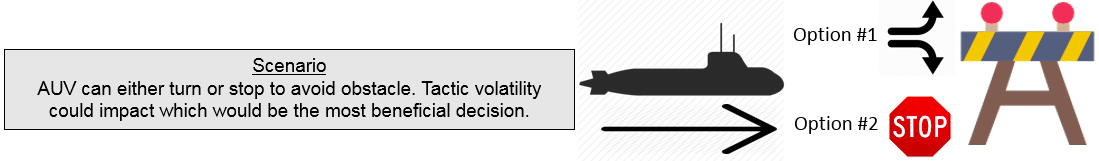
\includegraphics[scale=0.55]{images/AUVObstacle.png}
%    
\includegraphics[scale=0.55]{images/dummy.png}
%    \caption{XXXXXX}
%    \label{fig:AUVPingBaseStation}
%\end{figure}

%In the first example of this scenario, we will assume the following:

% DK: Probably change into a table
%\begin{itemize}[noitemsep]
%    \item \textbf{Benefit:} High -- The AUV will have a better understanding of base station response time and availability.
%    \item \textbf{Risk:} Low -- System is operating in a trusted environment
%    \item \textbf{Resource Cost:} Low -- A basic communication with the base station is energy inexpensive and creates little chance of component failure
%    \item \textbf{Current Uncertainty:} High -- AUV hasn't attempted to communicate with base station for quite some time 
    
%\end{itemize}

% Table~\ref{table:AUVDecisionAttributes}

%\begin{table}[h]
%\begin{center}
%\caption{Description of Uncertainty for AUV\dan{clean this up}\dan{make format consistent with other tables}} % DK: Feel free to reword this 
%\label{table:AUVDecisionAttributes}

%  \begin{tabular}{l|l|p{9.9cm} } \hline
%  \begin{tabular}{l | l} \hline
% \toprule
%  \bfseries X & \bfseries Min \\ \midrule
%   	\bfseries Item & \bfseries Level & \bfseries Description \\ \hline
%   	\bfseries Benefit & High & The AUV will have a better understanding of base station response time and availability \\ \hline
%   	\bfseries Risk & Low & System is operating in a trusted environment \\ \hline
%   	\bfseries Resource Cost & Low & A basic communication with the base station is energy inexpensive and creates little chance of component failure \\ \hline
%   	\bfseries Current Uncertainty & High & AUV hasn't attempted to communicate with base station for quite some time \\ \hline

%    X & X  \\ %\midrule %\midrule
    
%\bottomrule
%   \end{tabular}
%  \end{center}
%\end{table}




%Based on the above criteria, the AUV should likely perform the uncertainty reduction tactic of `pinging' or communicating with the base station. This would provide a greater amount of confidence in the system's knowledge about the time required and ability to communicate with the base station. However, let's assume that the AUV is now operating in an untrusted environment where it has the objective of operating in stealth mode. We will also assume that each time the AUV attempts communication with the base station, it risks compromising its location to adversaries. Therefore the `Risk' of communicating with the base station will be set to $High$. Although the execution of this uncertainty reduction tactic would provide greater confidence and data to the decision-making process, the AUV would likely choose not to perform this task due to the elevated amount of risk. 


%\vspace{-3mm}\paragraph{Example: Server Farm }
As a motivating example, we will use a hosting system comprised of numerous web servers. This system encounters various forms of uncertainty ranging from actions taken by adversaries, to component failure. The system has several possible uncertainty reduction tactics that it may use to address these various forms of uncertainty. These are described below: %\dan{add in volatility}


% DK: Probably change into a table
\begin{enumerate}[noitemsep]
%    \item \textbf{XXXX:} XXX
%    \item Data more external data by activating sensors
    \item \textbf{Activate extra layers of security: }In some situations, the system may detect that it is likely under attack by malicious actors. To reduce uncertainty if actors are either bots or actual humans interacting with the system, one uncertainty reduction tactic could be to force users to use `CAPTCHA' when logging onto the website. While CAPTCHA's may add an extra layer of protection, it can also hurt the user's experience.

    \item \textbf{Reduce model drift uncertainty: }`Chaos monkey' is a commonly used tool that evaluates a system's resiliency. This reduces uncertainty about a system's ability to deal with system failure and allows for collecting other variable information (such as the amount of time necessary to recover from failure.) A potential risk of using this uncertainty reduction tactic, is that in the event of high sever load, then perhaps the tactic should not be enacted since it will take more servers offline, reducing the availability of possibly essential resources. This could adversely impact the performance/stability of the system. Therefore, this uncertainty reduction tactic should only be used when specific scenarios are met.

    \item \textbf{Restore server to non-compromised backup instance: }This tactic could reduce uncertainty on if a resource has been comprised. However, a drawback is that the server will be unavailable while it is being restored to a `safe' state. There is also a minor risk of the restore encountering problems, making the server unavailable while these issues are being resolved. Another consideration is that performing a system restore may take a variable amount of time and may carry various risks.
    
    
    %Additionally, there is a minor risk of the restore encountering problems and the server being unavailable while these issues are being resolved.

\end{enumerate}
 
% Table~\ref{table:AUVDecisionAttributes}

While each of these uncertainty reduction tactics can be beneficial to the system, each tactic is likely to incur a different cost or encounter risks. Thus, it is imperative for a self-adaptive system to carefully consider the possible use of uncertainty reduction tactics, as they may cause more harm to the system than good. To accomplish this, a \ul{robust dynamic Bayesian matrix factorization model} is necessary to help determine if/when each uncertainty reduction tactic should be invoked. For example, while running `Chaos Monkey' can reduce model drift uncertainty it can also incur many costs in the form of time to execute the uncertainty reduction tactic, risk and even energy cost. To determine if this uncertainty tactic should be used, a robust process for anticipating the costs, risks, availability and dependability of this should be used. Otherwise, the system will largely be making a blind decision using inaccurate data. %\dan{proof all of this}

% Another exmaple could be restoring a server to a safe state



%While each of these uncertainty reduction tactics can be beneficial, they can also be detrimental to the system due to the resource costs and risks they may incur.  Therefore, a \ul{robust dynamic Bayesian matrix factorization model} is necessary to help determine if/when each uncertainty reduction tactic should be invoked. For example, although activating the `captcha' feature to reduce \emph{context} uncertainty can be a beneficial tactic, it can adversely impact the user experience. Therefore the tactic should only be used when specific security criteria is met. Additionally, uncertainty reduction tactics may be in conflict with one another. For example, while running `Chaos Monkey' can reduce model drift uncertainty, this tactic can be detrimental if the system is concurrently performing the uncertainty reduction tactic of restoring VMs to a trusted state. These operations would be in conflict with one another since both would be removing resources. Therefore, this could lead to situations where the robustness and stability of the system was adversely impacted due to a lack of server resources. This scenario demonstrate how numerous internal and external factors impact the decision-making process of selecting, or even executing an uncertainty reduction tactic.

\vspace{1mm}
This project proposes a dynamic Bayesian matrix factorization model to address the following challenges in seamlessly and effectively integrating uncertainty reduction tactics into the self-adaptive process to \textbf{enable self-adaptive systems to make more informed decisions:} 

\begin{enumerate}[noitemsep]

%	\item Uncertainty generally cannot be completely removed from any situation or process. Therefore, it is essential to \ul{quantify the uncertainty} anticipated to be removed by the tactic. This information will be used in the decision-making process to determine if, and which uncertainty reduction tactic should be used by the system.
	
%	\item It is crucial to \ul{evaluate the trade-off} of implementing each uncertainty reduction tactic and consider the risk and cost of executing the tactic.

	\item Prior to executing an uncertainty reduction tactic, the system should properly \ul{anticipate the volatility of using the tactic}. This volatility could in terms of  cost, risk, latency time, or other variables. 

	\item It is essential to \ul{predict the impact} of each uncertainty reduction tactic to determine the overall benefit it will provide to the system in reducing uncertainty. % Dk: Might want to remove this one
	
%	\item The \hl{decision-support process} must seamlessly integrate into widely used self-adaptive processes such as MAPE-K to \ul{support wide-spread adoption.}

    \item Uncertainty reduction mechanisms must seamlessly integrate into existing self-adaptation processes such as MAPE-K to \ul{enable wide-spread adoption}.

\end{enumerate}


% DK: Should this be moved?
\vspace{-7mm}\paragraph{Uncertainty Reduction Tactics} Recent works have discussed and demonstrated the potential impact that uncertainty reduction tactics can have on self-adaptive systems~\cite{moreno2018uncertainty,esfahani2013uncertainty,mahdavi2016classification,Ramirez:2012:TUD:2666795.2666812, camara2017uncertainty}. These tactics are specifically designed to reduce uncertainty during the decision-making process. Unfortunately, the use of uncertainty reduction tactics is currently only conducted in an ad-hoc manner, with no considerations made to trade-offs in terms of costs and benefits. An example of an uncertainty reduction tactic in an AUV could be to test a critical mechanical component to ensure that it is properly functioning. Another example of an uncertainty reduction tactic in a web-based hosting infrastructure could be a server sending a message to another server to better understand availability and response time~\cite{Hielscher:2008:FPS:1504902.1504917}. Some of the existing uncertainty reduction tactics and the sources of uncertainty are shown in Table~\ref{table:ExistingUncertaintyReductionTactics}. Traditional \emph{adaptation tactics} differ from uncertainty reduction tactics in that adaptation tactics are actions taken by the system to achieve specific system or mission goals. Uncertainty reduction tactics are actions specifically conducted to reduce uncertainty.

\definecolor{LightGray}{gray}{0.90}
\begin{table}[h!]
\begin{center}
\caption{Defined Uncertainty Reduction Tactics~\cite{moreno2018uncertainty, esfahani2013uncertainty}}
\label{table:ExistingUncertaintyReductionTactics}
\begin{tabular}{| l | l | } \hline 

  \bfseries \cellcolor{LightGray}Source of Uncertainty& \bfseries \cellcolor{LightGray}Tactic \\ \hline

	Simplifying assumptions & Use analysis with higher fidelity \\ \hline
	 Noise & Change the sampling rate \\ \hline
 
	 \multirow{3}{6em}{Model drift} & Probe service/device not recently used \\ \cline{2-2}
 	& Turn probe/sensor on \\ \cline{2-2}
 	& ``Chaos Monkey''  - Random resource termination\\ \hline
%	Humans in the Loop & Humans for their state?????? \\ \hline
	Decentralization & Query other systems \\ \hline

   \end{tabular}
  \end{center}
\end{table}

\vspace{-0mm}\paragraph{Technical Innovation and Extension to the State of the Art}
This research will advance self-adaptive/autonomous systems in the following key areas: (A) Facilitate self-adaptive systems in making \ul{more informed decisions} (B) Enable self-adaptive systems to \ul{avoid decisions that lead to bad and erratic outcomes} (C) Provide \ul{greater certainty and predictability} to internal and external data, and actions conducted by the system.

The developed dynamic Bayesian matrix factorization model will be integrated into the MAPE-K adaptation control loop, providing the benefits of uncertainty reduction to numerous self-adaptive systems. While previous research has demonstrated the effectiveness of considering uncertainty in the self-adaptive process~\cite{calinescu2011dynamic, camara2017reasoning, esfahani2013uncertainty}, no known techniques conduct specific actions designed to reduce uncertainty. Although adaptation processes are able to reason and model about internal and external uncertainty, unfortunately these processes are not yet capable of conducting actions specifically designed to reduce uncertainty. While in many cases reducing uncertainty is not possible due to irreducible causes (unknown adversarial actions, unpredictable weather conditions etc..) in many situations uncertainty is reducible and therefore can be addressed by the self-adaptive system~\cite{moreno2018uncertainty}. The proposed work will address current limitations in uncertainty reduction in self-adaptive systems and \ul{extend the current body of knowledge} in several main directions: (I) The creation of a process to anticipate the costs and potential benefits of uncertainty reduction tactics, something that previous research has defined as a need~\cite{moreno2018uncertainty} (II) The inclusion of the dynamic Bayesian matrix factorization model for uncertainty reduction tactics in the MAPE-K architecture, which will enable wide-spread adoption (III) Evaluation of the benefit of uncertainty reduction tactics in the self-adaptive process.

%%% Extends in XX directions:
%   Inclusion of decision-support process to select the most apporpriate uncertainty reduction tactics
%   Evaluation of such tactics
%   Adaptation of MAPE-K architecture to inclusde such tactics

% ? Talk about how this will help support mission/system critical objectives

% Will lead to better knowledge of current and future environments, situations and scenarios
% 

% Although self-adaptive systems are capable of performing decisions, they have not been evaluated/created to perform actions that are merely suited to reduce \emph{uncertainty}, enabling greater confidence in the system's other decisions.

% Advance a variety of self-adaptive processes as uncertainty has widely been demonstrated to inhibit the decision-making process in self-adaptive systems{include many citations}

% What other works talk about why this is needed. Show how this is a defined need
% 


\vspace{-0mm}\paragraph{Relevance to Navy} 

% Help with system resiliency/effectiveness/ability to complete mission-critical tasks/operations

% The proposed research is highly relevant to both the Naval and civilian domains. 

Military systems frequently conduct system and mission critical operations; ones that require high levels of certainty. The proposed work will provide greater amounts of certainty with minimal impact on existing operations and functionality. Uncertainty is recognized to be detrimental in a wide range of AI, machine learning and autonomous domains~\cite{mahdavi2016classification, camara2017uncertainty, esfahani2013uncertainty}. Therefore, the proposed research in uncertainty reduction can also be \ul{potentially transformative to many other autonomous domains} (e.g., cybersecurity, AUVs, self-driving cars etc..), that utilize self-adaptive components. This work aligns with the objectives defined in the \emph{Naval Research and Development Framework}, specifically `Augmented Warfighter' and `Integrated \& Distributed Forces'. The outcome of this project may be integrated into a wide range of systems ranging from small cyber-physical systems to large UAVs and AUVs. 

\subsection{Technical Objectives}
The proposed dynamic Bayesian matrix factorization based process is the first known effort to incorporate uncertainty reduction tactics directly into the self-adaptive process. This work will create systems with lower levels of uncertainty, therefore enabling them to make more informed decisions that are much more likely to lead to optimal outcomes. This section will describe the technical objectives that this project will achieve. These include: (1) the dynamic Bayesian matrix factorization model, (2) integration of created process into the MAPE-K adaptation control loop, (3) A systematic evaluation of the developed process to demonstrate its benefits to a variety of autonomous systems in reducing tactic uncertainty.

\vspace{-4mm}\paragraph{Objective I: Dynamic Bayesian Matrix Factorization for Tactic Recommendations} Self-adaptive systems must autonomously make decisions using constantly changing data about their internal and external environments, and frequently fluctuating mission and system objectives. This perpetually fluctuating data may be impacted by changing mission objectives, internal and external environmental variables and events, and even attacks by opposing forces. Despite the large amounts of heterogeneous data encountered, it is imperative that the self-adaptive system continue to operate in a robust manner while accomplishing defined objectives. Unfortunately, this data frequently contains varying levels of uncertainty which could adversely impact the system's ability to make the most appropriate decisions. This uncertainty may include the accuracy of a sensor reading, the availability of a resources, or the time necessary to complete a task. To help cope with these challenges, a robust dynamic Bayesian matrix factorization model is needed to predict various attributes regarding the uncertainty reduction tactics to determine the appropriateness of executing the tactic. Some of the attributes associated with uncertainty reduction tactics include the resource cost, execution time, risk, availability of the tactic, and dependability of the tactic. To address these challenges, we will develop a \ul{\em dynamic Bayesian matrix factorization model} to analyze historical usage data to predict (I) If an uncertainty reduction tactic should be implemented (II) The anticipated volatility associated with each tactic (cost, time to execute etc...) %\dan{proof}

%needed to evaluate the uncertainty associated with each tactic (system operation), and select an uncertainty reduction tactic that is most appropriate to reduce this uncertainty. Some of the considerations that such a model should consider are (I) The age of the last observed data point (II) What is the cost/risk of conducting each uncertainty reduction tactic (III) The level of calculated uncertainty regarding a data point (IV) The critically of a data point (consider what other tactics may rely upon this data). To address these challenges, we will develop a \ul{\em dynamic Bayesian matrix factorization model} to analyze observed data to determine A) The level of uncertainty with a tactic B) Perform a cost/benefit analysis to determine which (if any) uncertainty reduction tactic is necessary to address this uncertainty. A primary challenge is that there may be both observable and latent factors that must be accounted for as appropriately as possible, as they could both have a substantial impact the most appropriate outcome. 

% Volatility to be predicted and considered
\vspace{-4mm}\paragraph{Volatility in Uncertainty Reduction Tactics}Uncertainty reduction tactics have several forms of volatility that must be accounted for in the decision-making process. Some of the forms of volatility that our dynamic Bayesian matrix factorization model will account for are listed below:

\begin{itemize}[noitemsep]
    \item \textbf{Latency: }The time required to implement a tactic is known as \emph{tactic latency}~\cite{Moreno:2018:FED:3208359.3149180,moreno2017adaptation}. %The execution of any tactic could impact concurrent and subsequent tactics.
    
    \item \textbf{Risk: }Every action carries a specific amount of risk. This could be in the form of making yourself more vulnerable to an attack by an adversary or the risk of leading to a component failure. This value will be highly domain specific,  as the same action in different systems and scenarios can carry vastly different risks.

    \item \textbf{Availability: }The measure of how frequently the uncertainty reduction tactic has been available for use.
    \item \textbf{Dependability: }The measure of how well an uncertainty reduction tactic correctly produces its expected functionality.
    \item \textbf{Cost: }The cost of performing a tactic could come in multiple forms. Some of which include energy, or wear and tear on a physical component. 
\end{itemize}

\vspace{-4mm}\paragraph{Objective II: MAPE-K Integration }Self-adaptive systems must be able to efficiently and effectively autonomously respond to a variety of foreseeable and unforeseeable internal and external events. This is commonly accomplished using the MAPE-K adaption control loop. Any proposed uncertainty reduction process should be easy to include in this loop to ensure wide-spread adoption. A challenging aspect of this inclusion is that the process should not (1) Place any unnecessary limitations on the system (2) Should not adversely impact the system's ability to make effective and efficient decisions (3) Should not require any substantial changes to the system outside of this control loop, (4) Should not be domain specific, and be generic enough to be applicable to a wide-range of systems. Additionally, it should minimally impact the components inside of the loop. {\bf The proposed process will be integrated into the popular MAPE-K adaptation loop, enabling wide-spread  adoption in existing self-adaptive systems.} The inclusion of an uncertainty reduction process in the MAPE-K loop will support the system's ability to autonomously include this critical task of uncertainty reduction in the its standard process.


% Data will be taken in during the M phase, while the developed support process will be included into the `A' phase. The `A' phase will use data from the `K' base to determine (I) the level of uncertainty (2) the most appropriate uncertainty reduction tactic to implement (3) if the trade-off of running the tactic is worth implementing it

%MAPE-K~\cite{kephart2003vision} is a popular adaptation control loop that is used in a variety of self-adaptive and autonomous systems. This adaptation loop collects information in the $Monitor (M)$ phase, and then uses the $Analyze (A)$ and $Plan (P)$ phases to determine the actions that should be performed in the $Execute (E)$ phase. The $Knowledge (K)$ component stores all information shared between the monitor, analyze, plan and execute functions. {\bf The proposed process will be integrated into the popular MAPE-K adaptation loop, enabling wide-spread  adoption in existing self-adaptive systems.} 


%%%%%%%%%%%%%%%%%%%%%%%%%%%%%%%%%%%%%%%%

\vspace{-3mm}\paragraph{Objective III: Component and System Evaluation:}We will systematically evaluate all developed project components individually and then collectively to ensure that all objects are being sufficiently met. During our evaluation, we will need to consider many aspects of the self-adaptive system. For example, we will need to ensure that any negative impacts of our proposed process on existing self-adaptive processes are minimal, and that we provide a sufficient benefit to the system. This phase is not only important for evaluating our proposed uncertainty reduction process, but for demonstrating its effectiveness in self-adaptive systems. %In addition to the evaluation of our developed process, we will also assess the benefits of including uncertainty reduction tactics in the self-adaptive process.


%Figure~\ref{fig:evolutionaryEvaluationProcess} provides an overview of our evolutionary process evaluation.

% Will need the evaluation to consider many aspects of the self-adaptive system
% Compare the outcome of our process against others that do not use it (this is stated in the task)
% Systemtially evaluated at each stage of development (maybe include the image for this here)


% Ability to choose the proper tactics
% Not impact the existing self-adaptive process
% Fast and effective decision-making
% Easily integrated into existing self-adaptive structures/processes



%% DK: Add back in if space allows
%\begin{figure}[h]
%	\centering
%    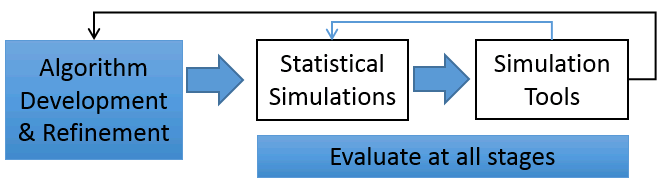
\includegraphics[scale=0.40]{images/EvolutionaryEvaluation.png}
%    \caption{Evolutionary Evaluation Process\dan{might remove this}}
%    \label{fig:evolutionaryEvaluationProcess}
%\end{figure}


% Evaluate both the XXX prediction model and its inclusion in 

% Evaluate in different environments using different sources of data
% Ability to include
% Will compare to systems that do not include our uncertainty reduction tactics. The data/mission objectives of each system will remain identical (except for the inclusion of these uncertainty reduction tactics)
% ?  Can our process handle the addition of new uncertainty reduction tactics
% 






\subsection{Related Research} % DK: I am not sure if we should have this section? Can cut this down if space is an issue
%\dan{Can remove this section if space is an issue}


%%% This should go someplace else
%\vspace{-3mm}\paragraph{Uncertainty Reduction Tactics.}
%XXXXX

% Describe current work in this area

% Could also add in a paper about volatility - Gabriel's PLC

\vspace{-0mm}\paragraph{Uncertainty in Self-Adaptive Systems.}
Uncertainty is generally considered to be detrimental to the self-adaption process, and can lead to decisions that create less than optimal benefit (utility)~\cite{calinescu2011dynamic, camara2017reasoning, esfahani2013uncertainty}. Uncertainty in self-adaptive systems comes in innumerable shapes and forms, and is by its very nature frequently unpredictable. Some examples of uncertainty include the precise actions of other drivers for a self-driving car, how an adversary may attempt to compromise an AUV, or even possible component failures. Uncertainty is detrimental since self-adaptive systems require accurate information to make well-informed decisions.

% Remove this if space is a major issue 
%Uncertainty can be grouped into internal or external categories. An example of external uncertainty for a AUV could be weather conditions. An example of internal uncertainty is determining the impact of an adaptation decision on the quality attributes of a system. Such an event could be determining the impact of replacing a software component to the system's responsiveness, or even on battery usage. As with humans, self-adaptive systems need accurate information to make well-informed decisions. Uncertainty has been shown to affect numerous areas of a self-adaptive system ranging from its decision-making effectiveness and efficiency, leading to directly impact the system's resiliency, robustness and ability to complete all mission objectives~\cite{mahdavi2016classification, camara2017uncertainty}. Uncertainty may be considered to be aleatory (due to variability or randomness) or epistemic (due to the lack of knowledge about the state of the system and not due to variability)~\cite{esfahani2013uncertainty}.
%\dan{likely remove this section or shorten it}
% DK: Check to see what is redudant with other sections


\vspace{-5mm}\paragraph{Uncertainty Reduction in Self-Adaptive Systems.}
% Describe how our work differs from other uncertainty reduction processes


Gabriel \etal\cite{moreno2018uncertainty} recently presented a formal set of \emph{uncertainty reduction tactics} in an effort to reduce uncertainty during the decision-making process. Uncertainty management in self-adaptive systems requires a process to both decent when to reduce uncertainty along with methods to reduce the various kinds of uncertainty that is encountered. Although some of the described uncertainty reduction tactics have been previously used~\cite{esfahani2013uncertainty,mahdavi2016classification,Ramirez:2012:TUD:2666795.2666812}, their use has been ad-hoc with no considerations made to tradeoffs in terms of costs and benefits. Some of the existing uncertainty reduction tactics are shown in  Table~\ref{table:ExistingUncertaintyReductionTactics}~\cite{moreno2018uncertainty, esfahani2013uncertainty}. % DK: Could probably add to this 




%% DK: I did not include this as I didn't feel like it would add much to this proposal
%\vspace{-5mm}\paragraph{Learning Support in Decision-making.}\dan{Qi: Write something here if you want}


\subsection{Technical Approach} 

\newcommand{\TA}{Uncertainty Reduction Using Dynamic Bayesian Matrix Factorization}
\newcommand{\TB}{MAPE-K Adaptation Control Loop Integration}
\newcommand{\TC}{Systematic Evaluation of Developed Framework}

\vspace{-2mm}
\addcontentsline{toc}{section}{Task 1: \TA}
\subsubsection{Task 1: \TA} \vspace{-2mm} 
% Does the benefit outweigh the cost of performing an action

We will create a machine learning prediction model to predict the uncertainty reduction tactic's volatility to recommend the appropriate usage of uncertainty reduction tactics. By learning from historical usage data of internal components and control algorithms, as well as environment features, the prediction model can anticipate an autonomous system's behavior in the near future along with needs and capabilities of uncertainty reduction. However, building such a prediction model faces several significant challenges. While various kinds of data can be collected through different channels, including onboard sensors, and through comms, there may be other {\em latent} factors that also affect the behavior of a system. These factors may be related to the systems' internal running status or something unexpected from the surrounding environment. They are referred to as {\em latent} because it is usually difficult to directly measure their values and the number of these factors also remains unknown. These latent factors may also change over time along with the running status of the autonomous system and its surrounding environment. Therefore, it is important to systematically capture these changes and their impact on the system's behavior. Additionally, since uncertainty comes in innumerable forms and can have a myriad of sources and impacts, it may be beneficial to construct a joint prediction model that can collectively predict all parameters. This would help to discover the dependency among variability and would make a more accurate and efficient prediction model.


%%% This is from Qi
%We will create a machine learning based prediction model to automatically and precisely quantify the tactic volatility in multiple key aspects including latency, dependability, and availability. By learning from the historical usage data of an autonomous system that covers both the characteristics of its internal components and control algorithms as well as features from the surrounding environment, the prediction model can anticipate the autonomous system's behavior in the near future. However, building such a machine learning prediction model faces several significant challenges. While various kinds of data can be collected through different channels, including onboard sensors and ground station that is in communications with autonomous system deployed in a field, there may be other {\em latent} factors that also affect the behavior of a system. These factors may be related to the systems' internal running status of or something unexpected from the surrounding environment. They are referred to as {\em latent} because it is usually difficult to directly measure their values and the number of these factors also remain unknown. These latent factors may also change over the time along with running status of the autonomous system and its surrounding environment. Therefore, it important to systematically capture these changes and their impact on the system's behavior. Additionally, since latency, dependability, and availability are interrelated and correlated, instead of building three separate prediction models, it may be beneficial to construct a joint prediction model that can collectively predict all three parameters. A joint prediction model can help discover the dependency among thees parameters besides making a more accurate prediction of their values. 


We will develop a {\bf dynamic Bayesian matrix factorization model that jointly predicts multiple correlated uncertainty parameters}. The joint prediction model assumes that there are a number of common factors, including both observable and latent, that affect these parameters. However, they may play a different role over different parameters. We will begin by modeling the latent factors and their contribution to the parameter of interest.

%%% This is from Qi
%We will develop a {\bf dynamic Bayesian matrix factorization model that jointly predicts multiple correlated volatility parameters}, including latency, dependability, and availability. The joint prediction model assumes that there are a number of common factors, including both observable and latent, that affect these parameters. However, they may play a different role over different parameters. We will begin by modeling the latent factors and their contribution to the parameter of interest. We will use latency as an example to derive its prediction model.  


Given multiple sequences of time series data for an autonomous system that records the latency values along with the measurable features, we represent a set of latent factors in a given sequence as a vector ${\bf r}_u\in\mathbb{R}^K$ and use another vector  $\boldsymbol{c}_u\in\mathbb{R}^K$ to denote the coefficients of these factors to the models parameters. To capture temporal dynamics, we propose a state-space model to capture the latent factors that evolve with time as well as sudden changes that are not directly related to the prior running status of the system and the previous state of its surrounding environment. 
\begin{align}
\nonumber\boldsymbol{r}_u^1\sim N(\boldsymbol{0},\zeta_u^{-1}I)\quad
& \boldsymbol{r}_u^t\sim N(A\boldsymbol{r}_u^{t-1},\eta_u^{-1}I) \\
\nonumber\zeta_u\sim Gamma(a_{\zeta},b_{\zeta})\quad
& \eta_u\sim Gamma(a_{\eta},b_{\eta})
%\end{displaymath}
\end{align}
The transition matrix $A$ can be treated in various ways. It can be set as simple as an identity matrix~\cite{Charlin2015dpf} or be learned as a full matrix that allows users' general preferences to more flexibly evolve~\cite{Sun2014}. Our approach falls in the middle by setting the transition matrix $A$ to diagonal. It mitigates the over-fitting problem from learning a full matrix while capturing some of the evolving trend of users' preference. Each entry $a_{kk}$ on the diagonal is assumed $ a_{kk}\sim N(1,\alpha^{-1}) $. For a given sequence, since the environment and the task for the system is typically fixed, we assume the weights of the latent factors remain stable over time and the dynamics of volatility, in this example latency, is introduced through the changes of the latent factors. 
\begin{align}
\nonumber\boldsymbol{c}_u\sim N(\boldsymbol{0},\phi_u^{-1}I)\quad\phi_u\sim Gamma(a_{\phi},b_{\phi})
\end{align}
 To capture the time-specific changes of the latent factors, we introduce a bias term at a specific time
\begin{align}
\nonumber b_u^t\sim N(0,\rho_u^{-1})\quad\rho_u\sim Gamma(a_{\rho},b_{\rho})
\end{align}
Finally, we use a vector ${\bf x}_u \in \mathbb{R}^D$ to denote the set of observable features and ${\bf w}_u \in \mathbb{R}^D$ to denote their weights. We place a Gaussian prior over ${\bf w}$: 
 \begin{align}
 {\bf w}_u \sim \mathcal{N} (0,A^{-1}), \quad A=diag(\alpha)
 \end{align}
By integrating impacts from both the latent and observable factors, a latency value at time $t$ is a drawn from the following distribution: 
 \begin{align}
 x^t_u \sim \mathcal{N}(\sum_k c^t_{uk} r_{uk}^t+\sum_d x_{ud}^tw_{ud}+b_u^t,\sigma)
 \end{align}
 
While we use latency as an example to derive the above modeling mechanism, it should be noted that the latent factors are jointly learned by simultaneously considering all parameters. So, the predictions of all forms of uncertainty reduction tactic volatility are conducted collectively by the single joint prediction model instead of several independent prediction models. Therefore, the proposed model falls into the general category of multi-task learning (MLK)~\cite{zhang2017survey}. While MLK has been intensively studied in the AI/machine learning communities, limited effort has been devoted to developing MLK models to analyze time-series data, with a few exceptions (e.g., \cite{wang2012high}). Besides simultaneously modeling multiple time-series sequences, the proposed model also collectively models both observed and latent features. This {\em hybrid model} best fits the special characteristics of a CPS as not all the features that affect its running behavior can be directly observed or measured. 

%Figure~\ref{fig:uncertaintyReductionProcess}

%\begin{figure}[h]
%	\centering
%    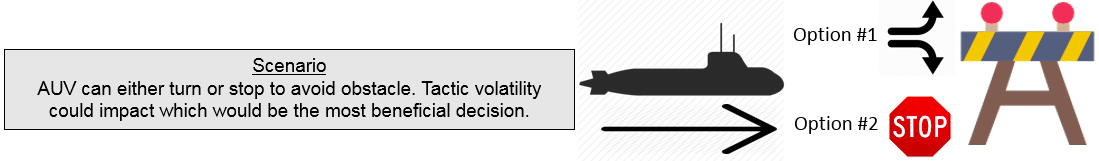
\includegraphics[scale=0.55]{images/AUVObstacle.png}
%    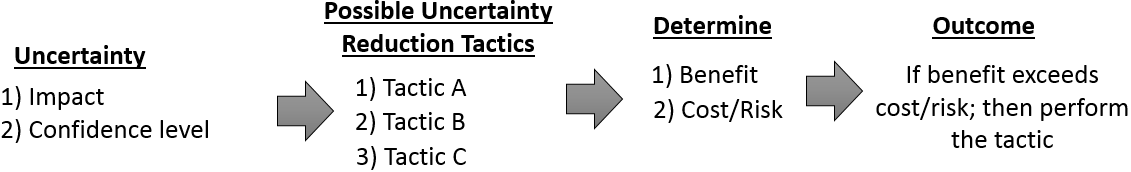
\includegraphics[scale=0.55]{images/uncertaintyReductionProcess.png}
%    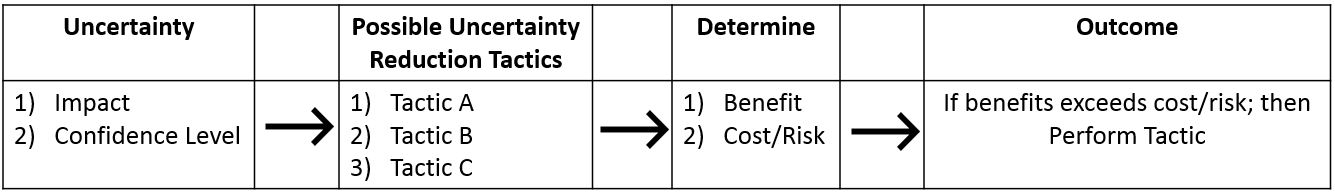
\includegraphics[scale=0.43]{images/uncertaintyReductionProcess2.png}
%    \caption{Overview of Proposed Process\dan{Make sure that this fits in with what is above}}
%    \label{fig:uncertaintyReductionProcess}
%\end{figure}




%\begin{center}
%\begin{tabular}{ |c|c|p{3cm}|c|c|c|c| } 
% \hline
% \textbf{Uncertainty} & -> & \textbf{Possible Uncertainty Reduction Tactics} & -> & \textbf{Determine} & -> & \textbf{Outcome} \\ \hline
% \begin{itemize}
%\item Improper Node/Node
%\item Improper Node/Node
%\end{itemize}
 
 
% & \raisebox{-\totalheight}{
\includegraphics[width=0.1\textwidth, height=15mm]{images/rightarrow.png}}
%    & cell6 \\ \hline
% cell7 & cell8 & cell9 \\ \hline
% \hline
%\end{tabular}




%\begin{table}
%\begin{tabularx}{\textwidth}{|>{\setlength\hsize{1.4\hsize}\setlength\linewidth{\hsize}}X|>{\setlength\hsize{.9\hsize}\setlength\linewidth{\hsize}}X|>{\setlength\hsize{.7\hsize}\setlength\linewidth{\hsize}}X|}
%\hline
%Types & Type of Critical Point & Stability \\
%\hline
%1. Real unequal eigenvalues of same sign
%\begin{itemize}
%\item $\lambda_1 > \lambda_2 > 0$
%\item $\lambda_1 < \lambda_2 < 0$
%\end{itemize} &
%\vphantom{1. Real unequal eigenvalues of same sign}
%\begin{itemize}
%\item Improper Node/Node
%\item Improper Node/Node
%\end{itemize} &
%\vphantom{1. Real unequal eigenvalues of same sign}
%\begin{itemize}
%\item Unstable
%\item Asym. Stable
%\end{itemize}\\
%\hline
%2. Real unequal eigenvalues of opposite sign
%\begin{itemize}
%\item $\lambda_2 < 0 >\lambda_1$
%\end{itemize} &
%\vphantom{2. Real unequal eigenvalues of opposite sign}
%\begin{itemize}
%\item Saddle Point
%\end{itemize} &
%\vphantom{2. Real unequal eigenvalues of opposite sign}
%\begin{itemize}
%\item Unstable
%\end{itemize}\\
%\hline
%3. Equal eigenvalues \newline Subtype 1: Two Independent vectors
%\begin{itemize}
%\item $\lambda_1 = \lambda_2 > 0$
%\item $\lambda_1 = \lambda_2 < 0$
%\end{itemize} &
%\vphantom{3. Equal eigenvalues} \vphantom{ Subtype 1: Two Independent vectors}
%\begin{itemize}
%\item Proper Node
%\item Proper Node
%\end{itemize} &
%\vphantom{3. Equal eigenvalues} \vphantom{ Subtype 1: Two Independent vectors}
%\begin{itemize}
%\item Unstable
%\item Asym. Stable
%\end{itemize}\\
%\hline
%\end{tabularx}
%\end{table}



% DK: This stuff could be cleaned up as it is largely restated later in Task #3
\vspace{1mm} \noindent \textbf{Evaluation of Task 1: }The effectiveness and benefits of the developed process will be systematically evaluated in an evolutionary manner using existing and created data sets. We will use existing data sets from The Internet Traffic Archive~\cite{InternetTrafficArchive_URL} and other sources such as SEAMS Exemplars~\cite{SEAMS_Exemplars_URL}. These existing data sets will enable us to develop, evaluate, and refine our process using real-world data that contains uncertainty. When necessary, we will also seed instances of uncertainty and volatility into the data sets. A comprehensive evaluation of all tasks is later described in Task \#3.


\addcontentsline{toc}{section}{Task 2: \TB}
\subsubsection{Task 2: \TB} \vspace{-2mm} 

%\addcontentsline{toc}{section}{Task 2: Integration into  MAPE-K Self-Adaptation Control Loop} 
%\subsubsection{Task 2: Integrate Proposed Process into MAPE-K Adaptation Control Loop} \vspace{-2mm}

The MAPE-K self adaptation control loop is extremely popular in self-adaptive systems~\cite{kephart2003vision, Iglesia:2015:MFT:2819320.2724719}. This self-adaptive process enables the system to autonomously react to internal and external events, along with changing mission objectives. The primary components of this loop are described below:

\begin{itemize}[noitemsep]
    \item \textbf{Monitor: }Collects observations from both internal and external environments. 
    \item \textbf{Analyze: }Performs complex reasoning and data analysis on data provided by the monitor function. In the event of required changes, this passes requests to the plan function.
    \item \textbf{Plan: }Selects or generates the necessary action(s) in the managed resource.
    \item \textbf{Execute: }Uses effectors to alter the behavior of the managed resource. Acts based upon the actions recommended by the plan function.
    \item \textbf{Knowledge Base: }Stores all information shared between the monitor, analyze, plan and execute functions. Generally created by monitor and frequently updated by execute. 
\end{itemize}

% DK: Might not be a bad idea to use an MDP in this demonstration

% Where we will integrate this process. Where does it fit into the loop
%   Are there any details we can provide for how we will be doing this

\vspace{-1mm}

We will integrate our dynamic Bayesian matrix factorization model into the \emph{Analyze} and \emph{Plan} stage of the MAPE-K adaptation control loop. Figure~\ref{fig:exampleMAPEK} provides a representation of the MAPE-K adaptation control loop, and where our process will be integrated into. 
\begin{figure}[h]
	\centering
   % 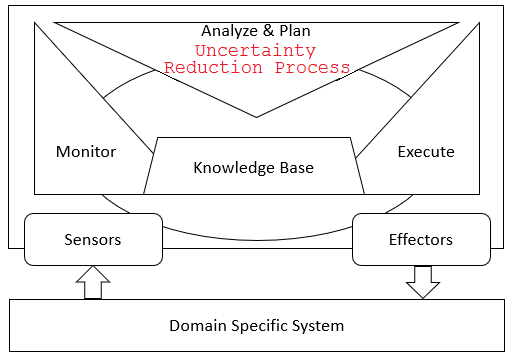
\includegraphics[scale=0.70]{images/mapek-uncertaintyreduction.png}
    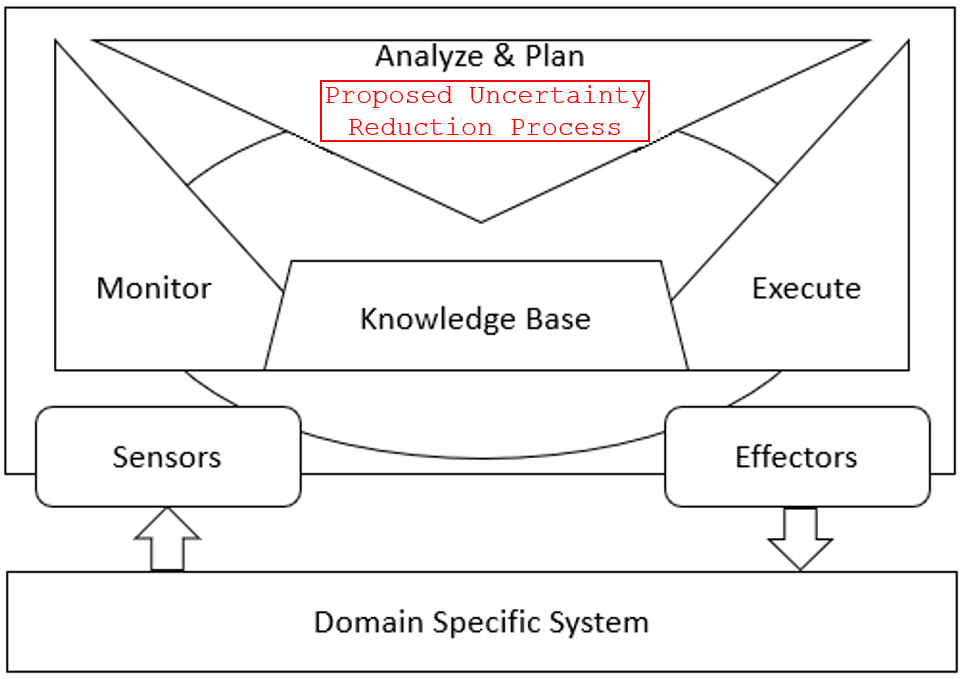
\includegraphics[scale=0.28]{images/mapek-uncertaintyreduction-2.png}
    \caption{MAPE-K with integrated dynamic Bayesian matrix factorization model}
    \label{fig:exampleMAPEK}
\end{figure}



% What is the process that we will use 
%   Mention the several different integration phases that we will use
% (Mention who will be responsible for what in the qualifications section - Be sure to update this in this paper along with the budget justification document that Laura sent out)


%%% Might need to move this
Our proposed Bayesian dynamic matrix factorization model will be systematically integrated into the MAPE-K self-adaptation control loop in several stages. The initial step will be to integrate our process into a simple, self-created implementation of MAPE-K. We will next use more robust evaluation environments such as SWIM~\cite{moreno2018swim} and RUBiS~\cite{Rubis_URL}. During each phase of integration, we will need to overcome several challenges. Some of the challenges include ensuring that the feedback collected is properly stored into the \emph{K} (knowledge) stage, and that it won't impact other concurrent or subsequent tactics that they system must conduct to fulfill its other goals. The outcome of this phase will include a functioning proof of concept example that will demonstrate the capabilities and benefits of our proposed process.
%\vspace{1mm}

Although our work will primarily focus on the inclusion of the developed process into the MAPE-K architecture, we will also explore its use in other adaptation control loops such as Rainbow~\cite{garlan2004rainbow}. This will further demonstrate the capabilities of our work to achieve wide-spread adoption and have a \ul{broad impact on numerous autonomous and intelligent systems}.


% Ensure that it won't impact other concurrent or subsequent tactics that are more important by the system
% Do not inappropriately impact other system decisions (system must continue to operate correctly - effectively and efficiently)
% Feedback collected is properly stored into the K stage
% Proper sensor data is collected (?not sure how to quantify this?)




%We will systematically integrate our proposed process into MAPE-K in several stages. The initial step will be to integrate our process into a simple, self-created implementation of MAPE-K. We will next use more complicated, existing environments such as SWIM~\cite{moreno2018swim} and RUBiS~\cite{Rubis_URL}. %We will evaluate our proposed technique using the evaluation criteria further described in Task \#3.





%%%% Challenges that need to be overcome
%   Be quick, efficient - Little impact on other decisions-actions
%   Must be seamlessly integrated: quick, efficient - Little impact on other decisions/actions. Enable the rest of the system components to continue to act effectively
%   The performed uncertainty reduction tactics must now adversely impact the concurrent or subsequent action of tactics that the system must perform (this might go into another section)

\vspace{2mm} \noindent \textbf{Evaluation of Task 2:} We will evaluate the ability of our proposed technique to be integrated into the MAPE-K self adaptation control loop in several manners. We will implement and evaluate our proposed technique into several self-created, and existing adaptation tools~\cite{moreno2018swim, Rubis_URL}. During each stage, we will evaluate (A) If our process can be properly implemented (B) The potential adverse impact that this process may have, specifically on the \emph{Monitor} or \emph{Execute} phases (C) The impact (positive or negative) on the system's efficiency, effectiveness and robustness. 

%The proposed \hl{decision-support} mechanism to be included in the MAPE-K will be evaluated based on its ability to be included in this adaptation control loop while provided all expected benefits, with little/no impact on the current processes being conducted by this loop. % DK: Clean this up

% Don't focus on the overall process, only how this one is evaluated.

% Evaluate in simulated environments, after the creation of small adaptation loops


%\addcontentsline{toc}{section}{Task 3: Data Creation} % DK: Rename this
%\subsubsection{Task 3: Data Creation} \vspace{-2mm}\dan{I am not sure if we will leave this task in.}

%   Create real-world data set that will enable evaluation of our process
%   Will also assist other researchers as well


%\vspace{1mm} \noindent \textbf{Evaluation of Task 3:} XXX

\vspace{-3mm}
\addcontentsline{toc}{section}{Task 3: \TC}
\subsubsection{Task 3: \TC} \vspace{-2mm} 

We will conduct a systematic evaluation to provide a demonstration of the capabilities of our proposed process to positively impact self-adaptive systems. Each step will be evaluated using both self-created data, and existing data from external sources such as `The Internet Traffic Archive'~\cite{InternetTrafficArchive_URL} and `SEAMS Exemplars'~\cite{SEAMS_Exemplars_URL}. Each step will be evaluated using the criteria defined below:

\begin{enumerate}[noitemsep]

  	\item \textbf{Increased System Resiliency: }It is imperative for self-adaptive systems to remain resilient in the face of unforeseen internal and external variability. We will evaluate the ability of our created process to enable systems to remain resilient when encountering volatility.

% DK: This could be added back in, but I feel like it is a boolean goal
%\item \textbf{Ability to be implemented into existing Self-adaptive architectures: }Proposed efforts must be able to be easily implemented in existing self-adaptive loops to support wide-spread adoption. By including the proposed pro

%   \item \textbf{Ability to be implemented into existing Self-adaptive architectures:} The success of this objective will be evaluated through the integration of our process into several existing self-adaptive devices.

     \item \textbf{Ability of Proposed Process to Assist in  System Efficiency: }A primary objective of self-adaptive systems to make efficient decisions. This efficiency could be defined in terms of time, or other system resources. Our created process should enable systems to make better, more efficient decisions. The proposed process must also be able to quickly make decisions and not impact the system's decision-making latency. The proposed process must also effectively evaluate the costs and potential trade-offs when executing an uncertainty reduction tactic to determine if and what tactics should be conducted by the system.

    \item \textbf{Support the Completion of Mission and System Critical Objectives: }Self-adaptive systems must frequently complete a wide-range of system and mission critical operations. Examples of system critical operations include an RPA activating an important cooling mechanism when engine temperatures reach a specific level, and an example of a mission critical operation could be the RPA assisting troops in contact. The proposed process must support the completion of these critical tasks in self-adaptive systems.

   \item \textbf{Evaluate Benefit of Each Uncertainty Reduction Tactic: }Although uncertainty reduction tactics have been proposed and defined~\cite{moreno2018uncertainty}, there is a lack of a thorough evaluation of each technique in various scenarios. We will measure and evaluate the benefits of the uncertainty reduction tactics in various simulated scenarios. While the goal of our work is not to serve as a conclusive, definitive guide for the evaluation of uncertainty reduction tactics; it will be the first known effort to evaluate such tactics.

\end{enumerate}

Using the above criteria, we will compare our proposed process to existing mechanisms that do not contain such a process to reduce system uncertainty. These evaluations will be conducted in a laboratory setting using R/MatLab, self-created MAPE-K adaptation loops, and in existing tools such as SWIM~\cite{moreno2018swim} and RUBiS~\cite{Rubis_URL}.


%In addition to demonstrating the potentially transformative impact of our proposed process, we will also conduct a systematic valuation of each uncertainty reduction tactic in the self-adaptive process to determine 

% What data will we use
% What steps will be done
% How will we measure success
% Compare our system with uncertainty reduction tactic to systems that do not include this (mention the different types of software that we will use - RUBIS, SWIM, etc....)
%   The differences between the evaluated techniques will help to demonstrate the effectiveness of our work

%SWIM~\cite{moreno2018swim} 
%RuBiS~\cite{Rubis_URL}


%\vspace{1mm} \noindent \textbf{Evaluation of Task 4:} >>> Probably not needed 


\vspace{-5mm}
\section{Project Schedule and Milestones}
As displayed in the following research schedule, the work will be conducted with many of the tasks operating in parallel:

 \newcounter{milestoneCounter} 
 \setcounter{milestoneCounter}{1}
% %% \addtocounter{milestoneCounter}{1}
% % \themilestoneCounter % How to call it
% %%%%%

\newcommand{\bLozenge}{\mathbin{\blacklozenge}}

\begin{table}[h]
\centering
\caption{Schedule of Proposed Project Events and Milestones}
\label{milestones}
%\begin{tabular}{|L{90mm}|l|l|l}|l}|l}|l|}
\begin{tabular}{|L{114mm}|L{3mm}|L{3mm}|L{3mm}|L{3mm}|L{3mm}|L{2mm}|}

\hline
\multirow{2}{*}{\textbf{Events and Milestones}} & \multicolumn{6}{c|}{\textbf{3-Year (1/2 Year blocks)}}               \\ \cline{2-7} 

% 6 month blocks

& 1 & 2 & 3 & 4 & 5 & 6 \\ \hline

Task \#1: \TA  & $\bLozenge$ & $\bLozenge$ & $\bLozenge$ & $\bLozenge$ & &     \\ \hline 
Task \#2: \TB  & & & $\bLozenge$ & $\bLozenge$ & $\bLozenge$ & $\bLozenge$     \\ \hline 
Task \#3: \TC  & & $\bLozenge$ & $\bLozenge$ & $\bLozenge$ & $\bLozenge$ & $\bLozenge$    \\ \hline 

 Documentation of findings                                       & & $\bLozenge$ & $\bLozenge$& $\bLozenge$& $\bLozenge$& $\bLozenge$  \\ \hline 

\end{tabular}
\end{table}

%\vspace{-5mm}
\section{Reports}
Required reports will be created adhering to NSWC/USN guidelines. These will also be made available to all relevant project stakeholders. The proposed work will produce several final outcomes, including:

%	Technical and Financial Progress Report
%	Final Report



\begin{enumerate}[noitemsep]
  \item Regular progress reports/meetings as desired by NSWC representatives.
  \item All project source code and other created artifacts.
  \item Results of all performed evaluations and demonstrations .
  \item All technical publications including conference and journal publications. 
  \item All evaluation data that demonstrates the evaluated study metrics.
  \item A prototype of developed process, including the inclusion in the MAPE-K adaptation loop.
  \item Financial Progress Report (as desired).
  \item Final report that discusses the final project outcomes, achieved objectives and future work.

\end{enumerate}



\vspace{-5mm}
\section{Management Approach}
PI Krutz and Co-PI Yu have a demonstrated record of success in collaborating on several research projects, as well as a funded DOD project. Their experience broadly provides all addressed research areas. Krutz will lead all efforts in the inclusion of the developed process in the self-adaptive process, along with all evaluation tasks. Yu will lead the development of the proposed Bayesian dynamic matrix factorization model.

\subsection{Facilities}
High performance computing is provided by Research Computing~\cite{RIT_ResearchComputing_URL} at RIT. This organization possesses six Sun Fire X4600 M2 servers with eight quad-core 2.3GHz AMD processors and 64GB of memory. Two Sun Fire X4500 servers that hold 48TB of raw data each are also available.



\section{Qualifications}


%PI Krutz and Co-PI Yu have a demonstrated record of success in research collaboration. The 

\vspace{-3mm}\paragraph{(PI Krutz - RIT)}is an Assistant Professor in the Department of Software Engineering and is affiliated with the Center of Cybersecurity. Krutz has authored over 27 publications, many of which focus on self-adaptive systems, or analysis and verification~\cite{McAfee:2017:CCA:3104086.3104132, Understanding_Relationship_SEAD18,Chester:2017:MLD:3104086.3104135, Dennis:2017:PPS:3104086.3104136,krutz2015examining, krutz2013cccd, krutzThesis}. Krutz has experience in the military domain having received an AFRL Summer Faculty Fellowship in 2018. Krutz holds a PhD in Computer Science, and a B.S. in History with an emphasis in military conflicts. He is experienced in leading software development projects, having worked as a software engineer in industry for over seven years.


\vspace{-3mm}\paragraph{(Co-PI Yu - RIT)}is an associate professor in the Department of Information Sciences and Technologies (IST). Yu's primary research interest lies in the fields of machine learning, AI, and data mining, with a special focus on dynamic data modeling, multimodal data fusion, and Bayesian nonparametrics. Yu has authored over 80 publications and regularly published in top-tier AI and data mining venues, such as IJCAI, ICDM, and TKDE. He is currenlty serving as the graduate program director of the IST department. 






\vspace{-3mm}
\section{Rough Order of Magnitude} For the three year project, .5 weeks summer support is requested for Krutz and Yu. Three (3) years of support is requested for a PhD student that will be jointly advised by Krutz and Yu.





% Break this down by year
\vspace{-0mm} 
%\noindent \textbf{Total Requested Amount \emph{(3 years)}: }\$XX,XXX

\noindent \textbf{Requested Amount: }Yr 1 –\$54,571, Yr 2--\$49,571, Yr 3--\$49,847; Total: \$153,989 


%Total Senior Personnel Request: Yr 1 –$XXXX, Yr 2--$XXX, Yr 3--$XXXXa


% Be sure to mention anything else we add in (travel)


% Mention SS
% 3 years PhD student support (advised jointly by PI Krutz and Co-PI Yu)


%\pagebreak
%\section{Section for Random Stuff that will be moved}







%%%%%%%%%%%%%%%%%%%%%%%%%%%%%%%%

\label{lastpage}
\cleardoublepage


\appendix
%\addcontentsline{toc}{section}{Appendix}
%\begin{appendices}
%\chapter{Some Appendix}


%% DK: Put onto a different page since it does not count against the page limit
\setcounter{page}{1}

%\addcontentsline{toc}{subsection}{Project Schedule}
\cfoot{\thepage}
\pagenumbering{roman}
%\section{Appendix}

%\input{sections/Appendix.tex}



%% I think the appendix goes before the bib. Otherwise, I could see people missing it
\newpage
\pagebreak
\addcontentsline{toc}{section}{References}
\bibliographystyle{plain}
\bibliography{refs}

\pagebreak


%\section{Attached CVs}
%\label{sec: attachedCVs}
%\vspace{-20mm}
\addcontentsline{toc}{section}{Attached CVs}
%   DK: Add these back in
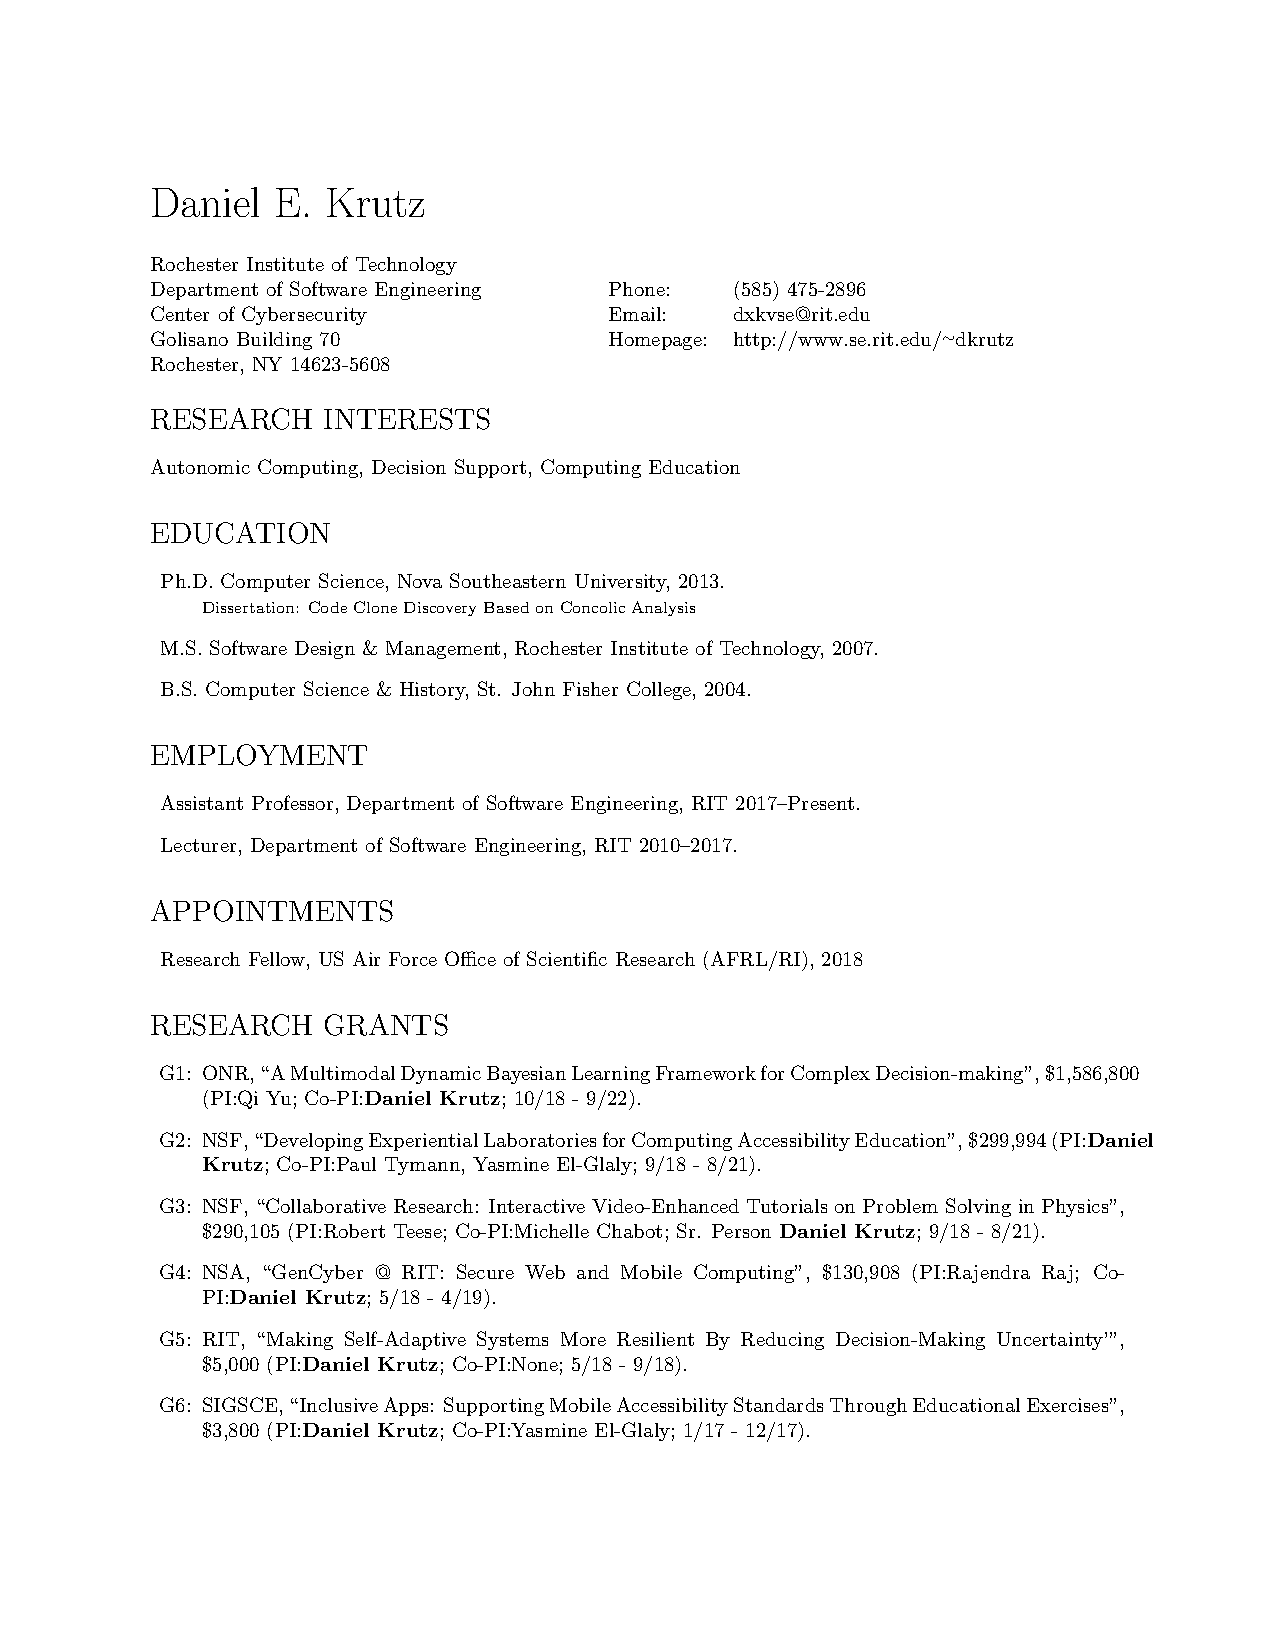
\includepdf[pages=-]{documents/cvs/Krutz_CVFull.pdf}
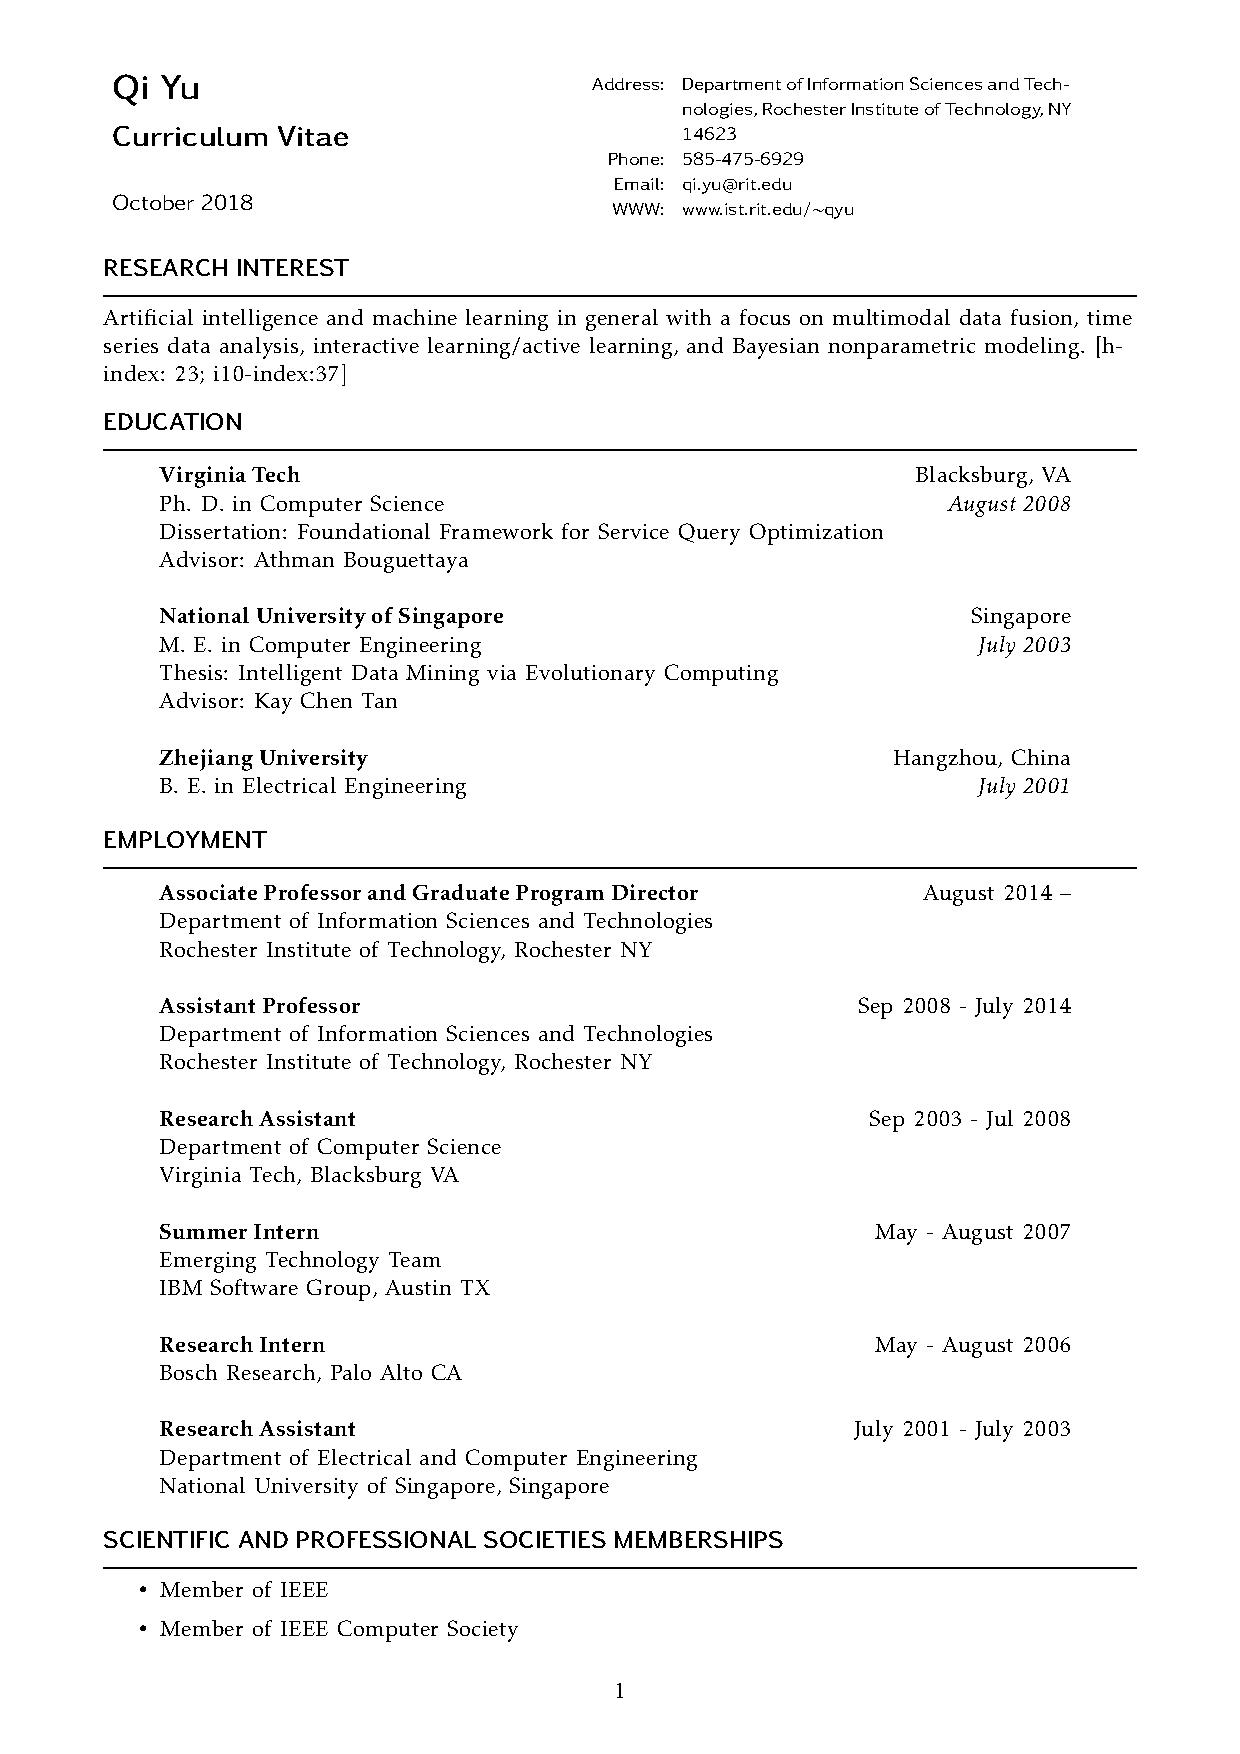
\includepdf[pages=-]{documents/cvs/Yu_CVFull.pdf}


\end{document}

% Paper on uncertainty reduction tactics: http://acme.able.cs.cmu.edu/pubs/uploads/pdf/seams18-ur-cr.pdf



% I've forwarded your document on to a few folks to see how interested they are but at first blush it appears interesting to have a method to have your AI tell you when it's likely going to make bad/erratic decisions. Please let me know if you have any questions.

%adaptation tactics—action primitives that change the system leaving it in a consistent state [13]

% [13] Shang-Wen Cheng and David Garlan. 2012. Stitch: A language for architecturebasedself-adaptation. Journal of Systems and Software 



% ? Can we add other types of volatility (from paper) into the equation



